%2multibyte Version: 5.50.0.2960 CodePage: 1251
\documentclass[11pt]{article}%
\usepackage{amssymb}
\usepackage{amsmath}
\usepackage{harvard}
\usepackage[mag=1000]{geometry}
\usepackage[doublespacing]{setspace}
\usepackage{amsfonts}
\usepackage{pstricks-add}
\usepackage{graphicx}
\usepackage{pgf}
\usepackage[pdftex]{graphicx}
\usepackage[nomarkers]{endfloat}

\setcounter{MaxMatrixCols}{30}

\providecommand{\U}[1]{\protect\rule{.1in}{.1in}}

\newtheorem{theorem}{Theorem}
\newtheorem{acknowledgement}[theorem]{Acknowledgement}
\newtheorem{algorithm}[theorem]{Algorithm}
\newtheorem{axiom}[theorem]{Axiom}
\newtheorem{case}[theorem]{Case}
\newtheorem{claim}[theorem]{Claim}
\newtheorem{conclusion}[theorem]{Conclusion}
\newtheorem{condition}[theorem]{Condition}
\newtheorem{conjecture}[theorem]{Conjecture}
\newtheorem{corollary}[theorem]{Corollary}
\newtheorem{criterion}[theorem]{Criterion}
\newtheorem{definition}[theorem]{Definition}
\newtheorem{example}[theorem]{Example}
\newtheorem{exercise}[theorem]{Exercise}
\newtheorem{lemma}[theorem]{Lemma}
\newtheorem{notation}[theorem]{Notation}
\newtheorem{problem}[theorem]{Problem}
\newtheorem{proposition}{Proposition}
\newtheorem{remark}[theorem]{Remark}
\newtheorem{solution}[theorem]{Solution}
\newtheorem{summary}[theorem]{Summary}
\newenvironment{proof}[1][Proof]{\noindent\textbf{#1.} }{\ \rule{0.5em}{0.5em}}
\geometry{left=1.1in,right=1.1in,top=0.75in,bottom=0.75in}
\usepackage{varioref}

\begin{document}

\title{Sticking to the Contract: \\Non-Profit vs For-Profit Banks and Hyperbolic Discounters\\(preliminary)\ \ \ \ \ \ \ \ \ \ \ \ \ \ \ \ \ \ \ \ \ \ \ \ \ \ \ \ \ \ \ \ \ \ \ \ \ \ \ \ \ \ \ \ \ \ \ \ \ \ \ \ \ \ \ \ \ \ \ \ \ \ \ \ \ \ \ \ \ \ \ \ \ \ \ \ \ \ \ \ \ \ \ \ \ \ \ \ \ \ \ \ \ \ \ \ \ \ \ \ \ \ \ \ \ \ \ \ \ \ \ \ \ \ \ \ \ \ \ \ \ \ \ \ \ \ \ \ \ \ \ \ \ \ \ \ \ \ \ \ \ \ \ \ \ \ \ \ \ \ \ \ \ \ \ \ \ \ \ \ \ \ \ \ \ \ \ \ \ \ \ \ \ \ \ \ \ }
\author{Karna Basu \& Jonathan Conning\thanks{Department of Economics, Hunter College,
City University of New York. Email: kbasu@hunter.cuny.edu,
jconning@hunter.cuny.edu. We are grateful to the Roosevelt House Public Policy
Institute and a Small Business Administration for initial research grant support. For
comments and suggestions, we thank Abhijit Banerjee, Eric Van Tassel, and
seminar and conference participants at Michigan State University, IIES
Stockholm, Delhi School of Economics, Queens College, Indian School of
Business, Hunter College, Florida Atlantic University, CIDE-ThReD Conference
on Development Theory, and NEUDC. Kwabena Donkor provided excellent research
assistance.}}
\maketitle

\begin{abstract}
Motivated by recurrent concerns about over-indebtedness and consumer protection
in microfinance and mortgage lending, this paper presents a model of lending
and refinance to hyperbolic discounters. First, we identify a problem of
consumer protection that survives even when consumers are sophisticated and
fully informed: a borrower would like to commit her future selves to a pattern
of repayments, but her future selves can be tempted to pay to defer debt
obligations via subsequent loan or refinancing offers. Investor-led banks may
find it costlier to credibly promise to enforce the commitment contract as has
an ex-post profit incentive to renegotiate its terms, limiting the amount of
commitment that can be offered in equilibrium. Second, we show how non-profit
and hybrid ownership (e.g. client or social investor-dominated)\ banks may
offer improved commitment. As organizations that face legal or governance
constraints that limit or bar these banks from distributing profits to outside
investors, they have a weaker incentive to renegotiate contracts, allowing
them to offer stronger commitment, ex-ante. Third, we show how a bank's
strategic choice to adopt non-profit or hybrid status depends on market
structure. A monopolist faces a trade-off: as a non-profit, it may earn higher
profits by providing superior commitment, but its ability to enjoy these
profits is restricted. Under competition, the trade-off disappears. If
contracts are exclusive, competition drives banks to adopt non-distribution
constraints. If contracts are not exclusive, for-profit banks will exist in
equilibrium and make superior commitment infeasible. The model helps explain
some stylized historical facts in consumer banking and recent developments in
microfinance. JEL Codes: O16, D03, D18\vfill


\end{abstract}

\qquad\newpage

\section{Introduction}

This paper analyzes the nature of equilibrium   and lending and saving contracts  in markets with hyperbolic discounters. We draw attention to
the demand for commitment in multi-period lending contracts, demonstrating
that there are circumstances where non-profit lenders -- or more broadly,
lenders that have chosen ownership/governance structures that place limits on
profit distribution -- can offer more effective and credible commitment
contracts than investor-led for-profit banks. A financial intermediary's
strategic choice to operate as a commercial non-profit or transform itself
into an investor-led for-profit firm depends on several factors, including the
extent of market competition, its ability to enforce exclusive contracts, and
the legal framework governing non-profits.

The model helps frame explanations for some important stylized facts about the
the operation of credit markets, including broad trends in the evolution of
ownership forms and issues of consumer protection in microfinance today, the
historical transformation of consumer finance in developed countries, and
consumer protection issues in mortgage refinance lending. \ In particular, the
model suggests a way to reconcile the following phenomena: the ubiquity and
persistence of non-profit and social-investor led firms in microfinance, and
the more recent growth of for-profit microfinance and its apparent association
with rising borrower `over-indebtedness' in some countries.

In recent years, especially in light of crises in consumer credit markets,
there has been renewed emphasis on consumer protection and better governance
and regulation in banking.\footnote{In the US, the Consumer Financial
Protection Bureau was set up in 2011 under the Dodd--Frank Wall Street Reform
and Consumer Protection Act. In India, the far-reaching Micro Finance
Institutions (Development and Regulation) Bill of 2012 was designed to
increase government oversight of MFIs in response to the credit crisis in the
state of Andhra Pradesh, and the perception that lax consumer protection and
agressive lending practices had led to rising over-indebtedness and stress.}
One particular area of concern has been borrower over-indebtedness, an issue
that has been at the center of recent microfinance repayment crises in places
as far-flung as Morrocco, Bosnia, Nicaragua and India. Commenting upon the
largest of these crises in the state of Andhra Pradesh in India, veteran
microfiance analyst Elizabeth Rhyne (2010) describes the build up of "rising
debt stress among possibly tens of thousands of clients, brought on by
explosive growth of microfinance organizations...\textquotedblright\ fueled by
the rapid inflow of directed private lending and new equity investors who,
because they \textquotedblleft paid dearly for shares in [newly privatized]
MFIs...\ needed fast growth to make their investments pay
off.\textquotedblright\ \ Her analysis, like that of many others ultimately
lays the blame on \textquotedblleft poor governance
structures.\textquotedblright\ \ Not too dissimilar descriptions have been
given to describe the build up to the 2008 mortgage lending crisis in the
United\ States. \ In each of these cases the issue of refinancings and/or the
taking of loans from multiple lenders emerges. For example, by value, more
than two-thirds of the subprime mortgage loans outstanding in 2008 were made
up of refinanced loans (Demyank and Van Hemert, 2009).

Journalistic and scholarly analyses of such situations, including the recent
mortgage crisis in the United States, have often framed the issues as problems
of consumer protection, suggesting that many lenders designed products to
purposefully take advantage of borrowers who have limited financial literacy
skills and are naive about their self-control problems. Informed by such
interpretations, new regulations introduced in the wake of these crises have
swung toward restricting the terms of allowable contracts, for example by
setting maximum interest rates, and the use of `coercive' loan recovery methods.

We place consumers' struggles with intertemporal self-control issues at the
center of the analysis but argue that borrowers are often more sophisticated
in their understanding of their own time-inconsistency than is often assumed.
From this perspective, `predatory lending' is not primarily about tricking
naive borrowers into paying more than they signed up for with hidden penalties
or misleading interest rates quotes, but about offering excessive flexibility
and refinancing of financial contracts in ways that limit or undermine the
commitments to long term consumption and debt management paths that borrowers
themselves may be attempting to put in place. \ A sophisticated hyperbolic
discounter understands that his `future selves' will attempt to take out new
loans on top of old ones, or renegotiate the terms of existing loans to
further defer debt repayment. That such borrowers should be and are willing to
pay for commitment has been demonstrated in several theoretical and empirical
papers.\footnote{A `sophisticated' hyperbolic discounter is one who is fully
aware of her time-inconsistency. See, for example, Ashraf, Karlan, and Yin
(2006), Carrillo and Dewatripont (2008), Bryan, Karlan, and Nelson (2010),
Fischer and Ghatak (2010), Basu (2011), and Basu (2012).} By entering into a
loan contract that commits them to a specific time-path of repayments, the
consumer atempts to ensure that future selves will not skew consumption
patterns to privilege instant gratification in the following periods. Viewed
this light, fees and punishments for failing to adhere to a repayment schedule
are not inherently undesirable to the consumer--for sophisticated hyperbolic
discounters, threats of punishment can indeed serve as useful commitment devices.

Nevertheless, the fact that consumers value commitment does not automatically
imply that firms will provide it in equilibrium. In fact, there remains an
open question about whether markets can be relied upon to supply commitment.
The key consideration is the following: if a hyperbolic discounter is willing
to pay to commit her future selves, her future selves are willing to pay to
undo this commitment. Here, a lender that promises to be rigid and is then
flexible could be seen as hurting, rather than helping, the
consumer.\footnote{Some recent papers demonstrate how commitment can be undone
in related settings. Gottlieb (2008) shows how competition leads to
inefficient outcomes in immediate rewards goods. Heidhues \& Koszegi (2010)
study the mistakes of partially naive borrowers in competitive credit markets.
Mendez (2013) analyzes predatory lending with naive consumers. We extend our
focus to monopoly, which is a particularly relevant market structure for
informal banking in developing economies, and study how the firm's governance
interacts with the renegotiation problem.}

Perspicacious readers will recognize that the idea that firm ownership might
be strategically chosen to solve or ameliorate `contract failure' problems
dates back at least to Arrow (1963)\ and one that has been articulated most
clearly in the work of Henry Hansmann (1980, 1996). \ Hansmann argued that in
markets where the quality of a product or service might be difficult to verify
clients may rationally fear that investor-led firms may be tempted to
opportunistically skimp on the quality of a promised product or service or
reveal a hidden fee, and this can greatly reduce or even eliminate
contracting. \ In such circumstances becoming a `commercial non-profit' may be
a costly but necesary way to commit the firm not act opportunistically, hence
enabling trade. \ Hansmann gives as a primary historical example the
development of consumer saving, lending and insurance products in the United
States and Europe. \ Life insurance in the United States for example has until
quite recently always been dominated by mutuals. \ Rate payers could not trust
investor-led firms to not act opportunistically for example, by increasing
premiums or by skimping or reneging on death benefit payouts. \ Mutuals on the
other hand had little incentive to cheat clients to increase shareholder
dividends as the clients themselves are the only shareholders. Mutuals
therefore enjoyed a distinct competitive advantage until sufficient state
regulatory capacity developed.

In the present analysis we begin by following Hansmann in defining non-profits
by the legal restrictions faced by them, setting aside other ways (such as
motivation) in which they might be different from for-profit
firms.\footnote{Hence we abstract away from other considerations for
nonprofits, as in Besley \& Ghatak (2005) and McIntosh \& Wydick (2005).
Nonetheless our modeling framework can be adapted to include these
considerations and is the focus of related work.} In this view "[a] nonprofit
organization is, in essence, an organization that is barred from distributing
its net earnings, if any, to individuals who exercise control over it, such as
members, officers, directors, or trustees. By `net earnings' I mean here pure
profits--that is, earnings in excess of the amount needed to pay for services
rendered to the organization.\textquotedblright\ Glaeser and Shleifer (2000)
and others have formalized Hansmann's central argument to show that when a
firm cannot commit to maintaining high quality, it might choose to operate as
a commercial nonprofit rather than as an investor-led for-profit in order to
credibly signal that it has weaker incentives to cheat the consumer on aspects
of unobserved product quality. As Hansmann describes it, firm ownership form
adapts endogenously as a `crude form of consumer protection' in unregulated
emerging markets where asymmetric information problems are rife. Bubb and
Kaufman (2011) modify this model so that the non-contractible quality issue is
on hidden penalties, which are incurred with certainty by some borrowers.
\ All of these models are built rely on some form of asymmetric information or
contract verification problem.

An important contribution of our paper is to argue that a theory of ownership
form can be built on behavioral microfoundations even in environments with no
asymmetric information and with sophisticated forward-looking agents. \ We
believe this is an important element for understanding the development of
consumer finance in developed countries historically as well as the current
shape of microfinance today where non-profit and `hybrid' forms still dominate
the sector in most developing countries (Cull and Morduch, 2009; Conning and
Morduch, 2011). \ `Hybrid' ownership forms include the many microfinance firms
that though technically incorporated as for-profit financial service providers
are in fact dominated by boards where, by design, social investors\ and/or
client representatives exert substantial governance control. \ Hybrid forms
such as these would appear to confer many of the benefits of non-profit status
(specifically, credible commitment to consumer protection) with fewer of the
costs (in particular, unlike a pure non-profit they can and do issue stock to
outside investors although usually in a manner that does not lead to challenge
control).\footnote{She goes on to argue that but for bad regulatory law
design, Indian MFIs might have avoided their problems and followed the model
of leading microfinance organizations in other countries like Mibanco and
Bancosol (Bolivia) which "were commercialized with a mix of owners including
the original non-governmental organization (NGO), international social
investors (including development banks), and some local shareholders. The NGOs
kept the focus on the mission, while the international social investors
contributed a commercial orientation, also tempered by social mission. In
Indian microfinance, NGOs are prohibited from becoming shareholders... [and
while clients may be given] a monetary stake in the company .. voting rights
[remain with] the founder/managers. At the same time, foreign investment rules
have made it hard for international social investors to participate in
ownership and governance. The results: founder domination, a pattern that
affects each of the big three MFIs in Andhra Pradesh and leads to a lack of
checks on decisions by managers..." \ Given that and "the entrance of pure
commercial players like Sequoia Capital India" \ it is not surprising to see
an "over-emphasis on fast growth" and a rise in consumer protection
complaints.}

In our earlier mention of the recent crisis of Andhra Pradesh which quoted
Elizabeth Rhyne at length because the rest of her analysis, which ties the
issue of financial intermediary ownership form and their lending pracices,
fits nicely into the framework of our model. \ In her view Indian MFIs might
have avoided their problems and followed the model of leading microfinance
organizations in other countries like Mibanco and Bancosol (Bolivia) which
\textquotedblleft were commercialized with a mix of owners including the
original non-governmental organization (NGO), international social investors
(including development banks), and some local shareholders. The NGOs kept the
focus on the mission, while the international social investors contributed a
commercial orientation, also tempered by social mission.\textquotedblright%
\ These are the types of hybrid ownership forms that we shall argue provide
the types of surplus building consumer protection that earlier theory argued
would be supplied primarily by non-profit forms. \ According to Rhyne,Indian
regulatory frameworks and policy decisions made it difficult for effective
hybrid ownership/governance structures to emerge
organically:\ \textquotedblleft In Indian microfinance, NGOs are prohibited
from becoming shareholders... [and while clients may be given] a monetary
stake in the company .. voting rights [remain with] the founder/managers. At
the same time, foreign investment rules have made it hard for international
social investors to participate in ownership and governance. The results:
founder domination, a pattern that affects each of the big three MFIs in
Andhra Pradesh and leads to a lack of checks on decisions by
managers...\textquotedblright\ \ With a flood of easy debt funding and
\textquotedblleft the entrance of pure commercial players like Sequoia Capital
India\textquotedblright\ the \textquotedblleft over-emphasis on fast
growth\textquotedblright\ and rising borower indebtedness and consumer
protection complaints becomes easier to explain.

As we explain below, non-profit or hybrid status firms can serve a useful
purpose even in the absence of contract failure -- the non-profit status
allows them to credibly promise to not renegotiate the terms of a commitment
contract. While the lessons in our paper apply to a wide range of contracts,
our focus is on lending. This modeling approach has the advantage of
generating a number of potentially interesting insights about the shapes of
equilibrium lending contracts.

\bigskip

[cite mendez predatory lending paper]

[Broad tables to show nonprofit/for-profit competition/monopoly around the world?]

[other reasons for nonprofit: http://www.nytimes.com/2015/03/03/business/some-private-colleges-turn-a-tidy-profit-by-going-nonprofit.html]

\bigskip

bullet points from slides:

\begin{itemize}
\item This is a paper about consumer protection in banking:

\begin{itemize}
\item How does a bank endogenously choose governance structure in response to
a consumer protection problem?

\item How does market structure affect bank's choice?
\end{itemize}

\item Standard concerns in consumer protection: hidden fees, bank's moral hazard.

\item We focus on a relatively under-studied problem: the provision of
commitment to time-inconsistent agents.

\item What kind of ownership and market structure helps banks offer credible commitment?

\item Motivating stories:

\begin{itemize}
\item Mortgage crisis

\item Microfinance: MFI explosion, apparent over-indebtedness, switch to
for-profit status
\end{itemize}

\item Two-part motivation:

\begin{enumerate}
\item For a time-inconsistent borrower, what matters in a loan contract?
Broader notion of consumer protection to include a dynamic commitment problem.
How does a bank commit to not renegotiate the terms of the contract?

\item How does the ability to commit vary based on governance and degree of competition?
\end{enumerate}

\item Key ingredient: Time-inconsistent individual's commitment motives are at
odds with same individual's future motives to undo commitment. For a consumer
to pay for commitment, firm must credibly commit to not undo it.
\end{itemize}

\bigskip

\begin{description}
\item Motivation 1 -- The Commitment Problem

\begin{itemize}
\item \textit{Commitment device}: contract that alters future action sets or payoffs associated with future actions.

\begin{itemize}
\item Make savings illiquid (fixed deposits)

\item Carrillo \& Dewatripont (EJ, 2008) -- promises that are costly to break,
asymmetric information

\item Fischer \& Ghatak (2010) - frequent repayment raises maximum
incentive-compatible loan size

\item Threaten punishment for non-repayment of debt
(microfinance--Banerjee--consumption transformation; Roscas--Basu, AEJ:Micro, 2011)
\end{itemize}

\item Growing literature that argues that time-inconsistency and commitment
matter, particularly in banking.

\item We will study this through the lens of loan contracts. Repayment embeds commitment.

\item Common focus of consumer protection/exploitation: (a) fees \&
punishments/naivete (Armstrong \& Vickers, JEL, 2012; Gabaix \& Laibson, QJE,
2006); (b) bank's moral hazard (Dewatripont \& Tirole, 1994; Oak \& Swamy)

\item But: sometimes consumers want punishments. Inability of bank to provide
\textit{credible} punishments should also fall under this umbrella. The
problem survives in the absence of naivete and asymmetric information.

\item The self being committed is willing to pay to rewrite the commitment
contract. Under what conditions would a bank renegotiate? We take seriously
the bank's ex-post considerations.
\end{itemize}

\bigskip
\end{description}

\begin{description}
\item Motivation 2--Market Structure \& Governance


\begin{itemize}
\item Ashraf, Karlan, \& Yin (QJE, 2006): "A natural question arises why, if
commitment products appear to be demanded by consumers, the market does not
already provide them."

\item We would like to see how market structure and governance interact with
the renegotiation problem.

\item Gottlieb (JPubET, 2008)--competition leads to inefficient outcomes in
immediate rewards goods.

\item Heidhues \& Koszegi (AER, 2010)--mistakes of partially naive borrowers
in competitive markets.

\item Monopoly should be taken seriously too, especially for development.
\end{itemize}
\end{description}

\begin{description}
\item Motivation 2a--Governance

\begin{itemize}
\item Hansmann (Yale Law Journal, 1980, 1987):

\begin{itemize}
\item "A nonprofit organization is, in essence, an organization that is barred
from distributing its net earnings, if any, to individuals who exercise
control over it, such as members, officers, directors, or trustees. By "net
earnings" I mean here pure profits--that is, earnings in excess of the amount
needed to pay for services rendered to the organization..."

\item "There is general scholarly consensus that the most convincing
efficiency rationale for employing the nonprofit form, as well as the apparent
reason why nonprofit firms in fact originally arose in most industries in
which they are found, is that the nonprofit firm serves as a crude but
effective consumer protection device in severe situations of asymmetric information."
\end{itemize}

\item Glaeser and Shleifer (JPubE, 2000): when a firm cannot commit to
maintaining high quality, it might choose to operate as a nonprofit rather
than a for-profit to credibly signal that it has weaker incentives to cheat
the consumer.

\item Bubb and Kaufman (2011): the non-contractibility is on hidden penalties,
which are incurred with certainty by some consumers, rather than quality.

\item We argue: similar analysis can be conducted in the absence of contract
failure or naivete. Instead: a renegotiation problem with fully informed and
optimizing consumers.

\item Analysis also sheds light on other structures, like social investors
(Conning \& Morduch, 2011).

\item \lbrack To focus on this problem, we abstract away from other
considerations for nonprofits--Besley \& Ghatak (AER, 2005), McIntosh \&
Wydick (2005).]
\end{itemize}
\end{description}

\begin{description}
\item Motivation 2b--Market Structure


\begin{itemize}
\item Rhyne (Huffington Post, 2010):

\begin{itemize}
\item ".. rising debt stress among possibly tens of thousands of clients,
brought on by explosive growth of microfinance organizations in southern
India. In the quest to meet their growth targets, loan officers often sell
loans to clients already indebted to other organizations."

\item "In many countries, leading microfinance organizations . . . were
commercialized with a mix of owners including the original NGO, international
social investors (including development banks), and some local shareholders.
The NGOs kept the focus on the mission, while the international social
investors contributed a commercial orientation, also tempered by social mission."
\end{itemize}

\item Broader notion of consumer protection: part of the "mission" is to limit renegotiation.

\begin{itemize}
\item Rigidity in traditional microfinance; refinancing flexibility with
credit cards and mortgage loans (credit card and mortage punishments gain
salience because they are\textit{\ less} strict, not more).
\end{itemize}

\item 1998-2006: Majority of subprime loans came from renegotiation (LA Times, 2008)
\end{itemize}
\end{description}

\subsection{Main Arguments}

In our model, there is no asymmetric information, so there is no uncertainty
of outcome or concern about deception via hidden actions or hidden information
in a contract. Instead, there is a renegotiation problem between fully
informed and optimizing agents. The issue is that after a loan contract is
signed and in effect, a present-biased borrower would, in a later period,
become interested in discarding the contract his period zero self had agreed
to and replace it with a new one that increases present consumption and pushes
repayment further into the future. Since at his later date the client will be
willing to pay to undo her earlier commitment, the bank (or perhaps one of is
competitors)\ might opportunisically pander to its clients impulses and
rewrite the existing contract to raise its profits. A sophisticated
consumer will anticipate this potential renegotiation in the initial period. In the
absence of an outside commitment technology the sophisticated bank and the
bank will search for second-best alternatives in renegotiation-proof loan
contracts, but this implies a reduction in the feasible contract space and
therefore in the total surplus or gains to trade that can be extracted. \ 

The bank's inability to commit to not pander to (i.e. not  profit
from) the client's later selves' temptation to recontract can therefore be
costly to the bank and this may lead it to explore commercial non-profit
status as a mechanism to more credibly commit to not opportunistically
exploiting the weaknesses of its time-inconsistent clients in that way. \ By
operating as a non-profit\ (or more broadly as a `hybrid' bank), the bank
agrees to face legal and/or governance restrictions on how any profits
generated from any such opportunistic renegotiation can be distributed and enjoyed

can more credibly convince the sophisticated consumer that it will be less
likely to renegotiate the contract in the future since the bank's managers and
outside investors now

. \ This allows the bank offer the consumer an initial contract that maintains
the restrictions on future consumption patterns that the consumer demands,
raising the contracting surplus and therefore how much can be ultimately
extracted by the bank's stakeholders. \ 

This argument is very similar in spirit to Henry Hansmann's (XXXX) explanation
for the existence of commercial non-profit firms. \ Note however that his
argument and later formalizations are built on the idea of consumers rational
fear that firms would try to deceive or otherwise opportunistically exploit
the environment of asymmetric information and/or costly enforcement. \ As
Hansmann himself `crude consumer protection'

A firm's decision about whether to adopt non-profit status rests on a
trade-off. As a non-profit, the firm has an opportunity to extract greater
surplus from the consumer (by providing commitment), but now faces
restrictions on the ability of managers and shareholders to enjoy this
surplus. This trade-off is sensitive to market structure. In the case of
monopoly, the bank will adopt nonprofit status if the following is true:
non-profit restrictions should be sufficiently severe that the bank is able to
extract more surplus from the consumer, but should not be so severe that it is
unable to enjoy the surplus.

Under competition, a lender's ability to provide effective commitment through
non-profit status depends on the exclusivity of contracts. When long-term
contracts can be made exclusive, the trade-off disappears and all active firms
function as non-profits. This is because of the zero-profit condition--since
firms do not make profits anyway, there is nothing to lose from switching to
non-profit status. On the other hand, there are profits to be gained--if all
other firms are for-profit, a firm could make positive profits by offering
superior commitment as a non-profit (this is valuable even if its enjoyment of
these profits is limited).

When contracts are not exclusive, commitment generated through non-profit
status becomes impossible to achieve. Since non-profit firms would make zero
profits anyway, each firm has an incentive to switch to for-profit status so
it can take advantage of the opportunity to re-finance \textit{other} banks'
loans. As a result, for-profit firms must be active in equilibrium, and their
presence will eliminate the possibility of non-profit commitment.

This can partly explain a key difference between traditional non-profit
microfinance, which is rigid, and say commercial credit card lending which
offers refinancing flexibility (credit card punishments gain salience because
they are\textit{\ less} strict, not more).

In addition, our model provides a partial (though obviously incomplete)
explanation of trends in global microfinance: the proliferation of lenders
erodes the monopoly advantages (through commitment) gained by non-profit
status, which results in a competitive equilibrium where firms switch to
for-profits and commitment properties of contracts are weakened, resulting in
an apparent over-indebtedness.

The problem of consumer protection in banking has been primarily analyzed
through two channels: naive or uneducated consumers and their failure to
correctly anticipate fees and punishments (Armstrong \& Vickers, JEL, 2012;
Gabaix \& Laibson, QJE, 2006), and bank's moral hazard (Dewatripont \& Tirole,
1994). We argue that, given the growing evidence of time-inconsistent
preferences, a bank's ability to provide credible commitment should also fall
under this umbrella. Through this lens, the model can shed some light on
ongoing debates and stylized facts in both formal and informal credit markets.

\bigskip

bullet points from slides:

\begin{itemize}
\item Focus on the following problem of consumer protection -- consumers want
commitment -- firms want to provide commitment, but are constrained by
governance and market structure. Our question: how?

\item Map out equilibrium loan contracts under monopoly and competition (quite different).

\item Formalize the renegotiation problem.

\item We show how, when there are strategically behaving time-inconsistent
agents and profit-minded lenders, lenders might choose nonprofit status even
if there is no incomplete contracts problem.

\item Here, there is a renegotiation problem instead, and nonprofit lenders
might be able to credibly signal that they will not renegotiate (even if both
both the borrower and lender would like to) when for-profit lenders cannot.
(But: tradeoff)

\item Ability of firms to commit through nonprofit status depends on
exclusivity of contracts and degree of competition (perfect competition can be
good or bad, depending on exclusivity.)
\end{itemize}

\section{The Model: Assumptions}

\subsection{Consumers}

There are three periods, $t\in\left\{  0,1,2\right\}  $. In any period $t$,
the consumer's instantaneous utility is given by $u\left(  c_{t}\right)  $ for
$c_{t}\in$ $[0,\infty)$. The utility function is twice differentiable,
strictly concave, and satisfies $u^{\prime}\left(  0\right)  =\infty$. Given a
consumption stream $C_{t}=\left(  c_{t},c_{t+1},...,c_{2}\right)  $,
the consumer period-$t$ self's discounted utility in period $t$ is:
\[
U_{t}\left(  C_{t}\right)  \equiv u\left(  c_{t}\right)  +\beta\sum
\limits_{i=t+1}^{2}\delta^{i-t}u\left(  c_{i}\right)
\]
This describes quasi-hyperbolic preferences, with a hyperbolic discount factor
$\beta\in(0,1]$.\footnote{More generally, utility would also be discounted by
an exponential discount factor $\delta$, so that $U_{t}\left(  C_{t}\right)
\equiv u\left(  c_{t}\right)  +\beta\sum\limits_{i=t+1}^{2}\delta
^{i-t}u\left(  c_{i}\right)  $. To streamline the analysis without loss of
generality, we assume $\delta=\frac{1}{1+r}=1$} In any period, the individual
places greater relative weight on immediate present-period gratification than
his earlier selves did. The consumer could be sophisticated, naive, or
partially naive about the time-inconsistency of his preferences (O'Donoghue \&
Rabin, 2001). Our analysis will focus on the sophisticated agent, with
extended discussions to other types.

The period 0 consumer starts with claims to an existing arbitrary income stream
$Y_{0}=\left(  y_{0},y_{1},y_{2}\right)  $ over the three periods but will in general be interested in consumption via `own savings' or  financial contracting opportunities with others. In banking or `own-savings' technologies are absent or prohibitively expensive, the consumer's autarky
consumption stream $C_{0}^{a}(Y)$ is  just be the exogenous income stream
$Y.$  With available `own savings' strategies the consumer may be able to
construct a somewhat better smoothed autarky stream. \ However, as
a consumer with time-inconsistent preferences cannot trust his later selves to not undo his
preferred consumption choices, the stream will be the imperfectly-smoothed outcome of a strategic game between selves as explained in Basu
(2014). This creates the demand for commitment services via  contracts an outside financial intermediary, and this is the main focus of our analysis. \ For the present moment we take this
autarky option $C_{0}^{a}(Y)$ to be fixed and given, but later show how the main results
are only slightly modified when we treat it as endogenous.\footnote{Since a
sophisticated hyperbolic discounter is fully aware of his future preferences,
his autarky consumption stream will be a subgame perfect equilibrium of the
consumption-savings game played by the series of his time-indexed selves (each
with a slightly different objective function).}
\\ In the sections that follow we state our results for quite general assumptions
about the shape of the the instantaneous utility function $u(c)$ but
illustrate and provide exact results for the CRRA case $u(c_{t})=\frac
{c^{1-\rho}}{1-\rho}$ where parameter $\rho$ is closely related to the
elasticity of intertemporal substitution.\footnote{ \(\)\(\rho \text{ }\)is the elasticity
of intertemporal substitution when $\beta=1$ [** still same when \(\beta<1\)?**]} \ The appendix contains closed form solutions for the CRRA case and other technical details. 


\subsection{Banks}

The period 0 consumer has the option of contracting with one or many
banks, depending on the market structure. Each bank has access to funds that
can be withdrawn from other investments at opportunity cost $r$. For expositional simplicity in main text results below we assume $r=0$ and that the consumer's discount factor is
$\delta=\frac{1}{1+r}$ (which implies $\delta=1)  $ but this is without loss of generality and more formulas for arbitrary $r$ and $\delta$ are in the appendix.
Any financial contract between the consumer and the bank can be thought of as
the consumer giving up income stream $Y_{0}  $ in exchange for a preferred
consumption path $C_{0}=(  c_{0},c_{1},c_{2}) $. A financial
contract involves a  period 0 loan if the exchange i such that $c_{0}>y_{0}$ and a savings
contract if $c_{0}<y_{0}$. [CUT? For now we also assume that  that any new contract
must be initiated in period 0.
] 

We assume the bank can perfectly enforce feasible repayment plans, so the net present value
of its remaining profit stream in period $t$ is given by:
\[
\pi_{t}\left(  C_{t};Y_{t}\right)  \equiv\sum\limits_{i=t}^{2}
\left(y_{t}-c_{t}\right)   
\]
The bank offers a contract if and only if it can earn non-negative profits.

If the contract were to be renegotiated in period $1$, the bank will incur a nonmonetary cost, $\overline{\kappa}\geq0$, which could be interpreted to include a concern for reputation or some other impact on the social
preferences of its owners.\footnote{The bank could incur additional monetary
costs as well. However, we assume these to be $0$ as they can be netted out
and do not affect the analysis in any important way.} The bank fully knows the borrowers preferences and can tailor the contract by borrower type.

While the primary focus of this paper is on equilibrium contracts, not
welfare, we will make occasional reference to the hyperbolic discounter's
welfare  defined as the
discounted utility of the period 0 self, $U_{0}$ (for a discussion the choice of welfare measure see O'Donoghue-Rabin, 1999).


\section{Monopolist Bank}

In this section, we analyze the renegotiation problem when a sophisticated
present-biased consumer faces a monopolist lender. We first derive properties
of the benchmark equilibrium `full-commitment contract' in the absence of any
renegotiation possibilities. We then describe how the contract would change
when the consumer understands and anticipates the possibility of contract
renegotiation between his later-period self and the bank. Finally, we describe
conditions under which a lender might strategically choose to operate as a
commercial non-profit.

\subsection{Full-Commitment Contract}


The monopolist who can offer a full-commitment contract solves the following
problem:
\begin{align*}
&  \max_{C_{0}}\pi_{0}\left(  C_{0};Y\right) \\
\text{s.t. (PC) }  &  U_{0}\left(  C_{0}\right)  \geq U_{0}\left(  C_{0}
^{a}(Y)\right)
\end{align*}
Let the monopolist's full-commitment contract be denoted $C^{mf}$. At an optimum:
\begin{align}
  u^{\prime}\left(  c_{0}^{mf}\right)  =\beta\ u^{\prime}\left(  c_{1}
^{mf}\right)  =\beta\ u^{\prime}\left(  c_{2}^{mf}\right) \label{foc-monop}\\
  U_{0}\left(  C_{0}^{mf}\right)  =U_{0}\left(  C_{0}^{a}(Y)\right)
\label{BPC-monop}
\end{align}

Condition \ref{foc-monop} is the standard first-order necessary conditions
that marginal utilities of consumption be equalized across periods which, for our simplifying assumptions, imply that  $c_{1}^{mf}=c_{2}^{mf}=\overline{c}^{mf}$. Condition \ref{BPC-monop} is the consumer participation constraint that they
be no worse off by accepting the contract than under autarky. \ For the
CRRA\ case the FOC  imply $\overline{c}^{mf}=\beta^{\frac
{1}{\rho}}c_{0}^{mf}$ which, along with the participation constraint, allow for closed form solutions (see appendix). See Figure 1.

The terms of the optimal contract, and hence also the level of bank profits, will  depend on the consumer's starting income stream \(Y_{0}\).   To see this, consider the set of possible initial income streams of constant present value   $\sum_{t=0}^{2}\frac{y_{t}}{(1+r)^{t}}=\bar{y}$. 

\begin{figure}[p]
\centering 
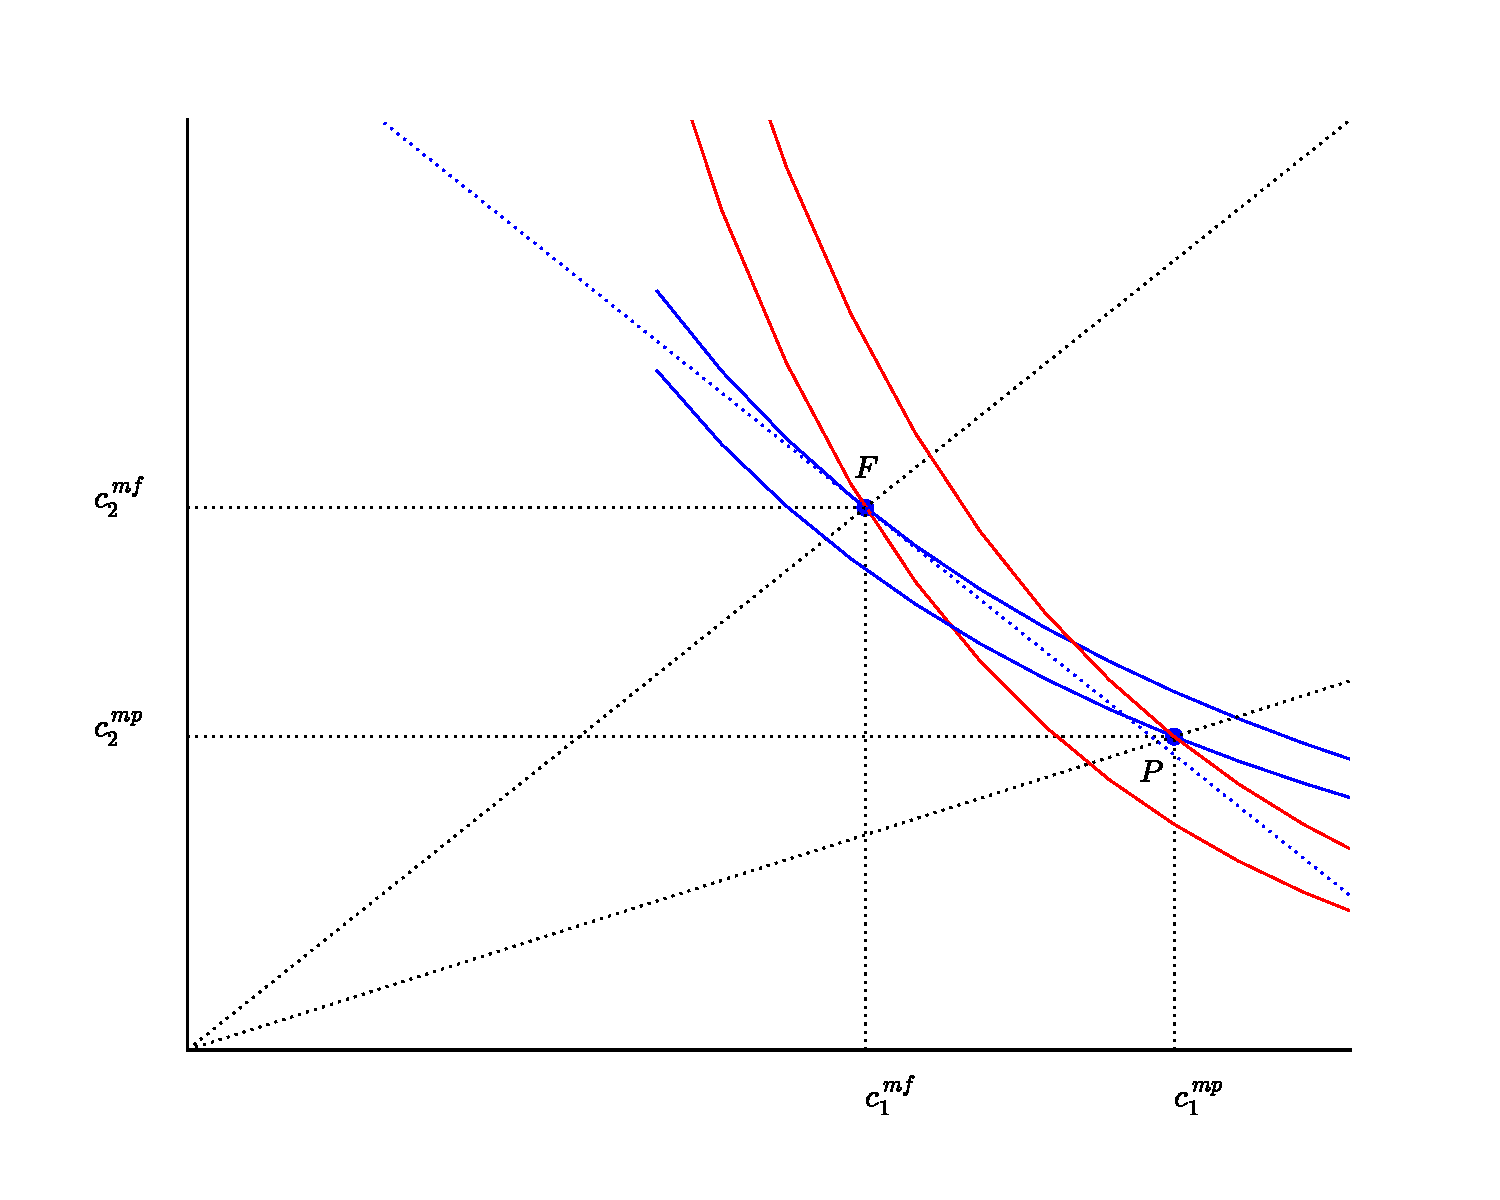
\includegraphics[scale=0.60]{MonopolyFig.pdf} 
\caption{Monopoly full-commitment contract in \(c_{0}\)\(-c_{1}\) space.}
\end{figure}
 

\subsection{The Risk of Renegotiation}


Bank  profits can be thought of as deriving in part from  satisfying the customer's `demand for commitment.' That is to say, the bank can charge for helping customers  to stick to preferred saving accumulation \textit{cum} loan repayment plans to deliver balanced consumption across periods 1 and  2 if it can credibly promise to not pander to the customers' later self's demands to raid savings and/or take out new loans that would disrupt those plans.

Figure 2 which is  drawn in $c_{1} -c_{2}$ space  illustrates why the demand for commitment arises, how a monopolist could profit by reneging on such a commitment \textit{ex-post} and therefore why a monopolist might take costly actions to try to make such commitments  more credible \textit{ex-ante}. Point $F$ is the balanced consumption  (\overline{c}^{mf},\overline{c}^{mf} )$ component of the monopolist's optimal contract. At this point period 0 consumption is $c_{0}^{mf}$ and participation constraint (\ref{BPC-monop}) is satisfied.  The flatter indifference curve passing through point \(F\) represents the customers' period-0 self's preference $u(c_{1}) + u(c_{2})$} to give equal weight to period 1 and period 2 consumption (in period 1 utils ) while line $NF$ can be interpreted as the isoprofit line associated with the monopolist's maximum profits from period 1 forward.

The demand for commitment arises from the fact that the period 0 self understands that as soon as period 1 rolls around his preferences will change and their period 1 self will now accept renegotiated contract offers to raise period 1 consumption even if this comes at the cost of period 2 consumption and period 0's discounted utility.\footnote{Measured in period 1 utils, Period 0 self values consumption bundle $(c_{1},c_{2})$ as $u(c_{1}) + u(c_{2})$ whereas period 1 self values the same bundle as $u(c_{1}) + \beta u(c_{2})$} Period 1 self values any bundle $(c_{1},c_{2})$ as $u(c_{1}) + \beta u(c_{2})$ period 1 utils whereas his earlier period 0 self valued the same bundle as as $u(c_{1}) + u(c_{2})$ period 1 utils.  Hence at contract point $F$ in the figure we have
\[
u^{\prime}\left(  c_{1}^{mf}\right)  \geq\beta u^{\prime}\left(  c_{2}
^{mf}\right)
\]

If he is a hyperbolic discounter with $\beta<1$, he wishes to increase present
consumption. As the figure illustrates, a monopolist can opportunistically `exploit' a customer who had agreed to $F$ by offering consumption stream $R$ in exchange for $F$. This would raise period 1 consumption by 'raiding savings' (taking out new loans), for a customer who had saved (borrowed) in period 0 by with the effect of lowering (increasing) the net savings (debt) passed into period 2.

FIGURE: Monopoly full-commitment contract in \(c_{1}\)\(-c_{2}\) space.}

Such a contract would be designed to raise period 1 self's utility ever so slightly while raising the monopolist to the higher value isoprofit line $QN$.  

This creates an opportunity for the bank to generate additional surplus. The bank might be willing to offer such a refinance, in
effect offering new loan and/or postponing repayments on  existing obligations or -- if the customer had carried savings into period 1 --  helping the customer `raid' savings for a fee. In such cases,
both parties voluntarily agree to renegotiate the original contract. 

A  sophisticated present-biased customer   anticipates such  potential renegotiations and will therefore only agree to renegotiation-proof contracts.   Since making contracts renegotiation proof only adds constraints to the contract design problem the monopolists' profits can only fall relative to the benchmark where it can costlessly commit itself to no renegotiations. The customer who was  already pushed against their autarky reservation utility is no worse off.  


More formally, consider the renegotiation problem that arises in period 1. A customer who has agreed to contract \(\hat C\)_{0}$\(  \) in period 0 enters period 1 with claims to remaining consumption stream $\hat C_{1}$. This determines the new reservation
utility. If profitable to  
the bank, the optimal renegotiated contract it offers will be given
by:
\begin{align*}
&  \max_{C_{1}}\pi_{1}\left(  C_{1};\hat C_{1}\right) \\
\text{s.t. }\text{}  &  U_{1}\left(  C_{1}\right)  \geq U_{1}\left(
\hat C\label{PCR}_{1}\right)
\end{align*}


The bank offers $C_{1}^{r}\left(\hat C_{1}\right)=\left(  c_{1}
^{r},c_{2}^{r}\right)  $ to replace\footnote{The bank swaps
net income stream ($y_{1}-\hat c_{1},y_{2}-\overline{}\hat c_{2})$ for
$(y_{1}-c^{r}_{1},y_{2}-c^{r}_{2}).$} the contractually agreed $(\hat c_{1},\hat c_{2}). $  Since the first-order conditions imply:
\[
u^{\prime}\left(  c_{1}^{r}\right)  =\beta u^{\prime}\left(  c_{2}^{r}\right)
\]the contract will set 
$c_{1}^{r}>$ $c_{2}^{r}$ as long as \(\beta<1 \) and exactly $c^{r}_{2}=\beta^{1/\rho} c^{r}_{1}$ in the CRRA case. Figure \FIGURE illustrates the type of renegotiated contract that would be offered in the very special case of a  customer who agreed to a full commitment contract $ C_{1}^{mf}$ in period 0 -- having sincerely believed the bank's promise to not offer to renegotiate in period 

1 --   was then genuinely and unexpectedly surprised to find the bank offering a renegotiation in period 1. Although it would break a promise to the consumer's period 0 self, the contract will be  designed to appeal to the customer's period 1. This type of renegotiation/promise-breaking will be profitable for the bank to offer  as long as $\pi_{1}\left(  C_{1}^{r}\left(  C_{1}^{mf}\right)  ;C_{1}^{mf}\right)  \geq\kappa$, where $\kappa$ are the non-monetary renegotiation costs to the bank. As depicted in Figure FIGURE, the bank will find it profitable to renegotiate from the   continuation of the full commitment  contract depicted by point $F$ to the new contract depicted by $B$ so long as profits gains (equal to the present value difference  between $ C_{1}^{mf}$ and $C_{1}^{r}$) which can be measured as  distance $NQ$ on the diagram is greater than $\kappa$.
 Although the new contract appeals to the period 1 self,  the broken promise  `exploits' the consumer's period 0 self by pushing their welfare below the autarky reservation utility that they thought had been promised by the $C_{1}^{mf}$ contract.  
 
\subsection{Renegotiation-Proof Contracts}

A sophisticated consumer will, of course, rationally anticipate the bank's temptation to break its commitment promises and for this reason would never   agree to accept contract \(F\)  or any other contract that could make him worse off following  a period-1 renegotiation. Since the bank will want to avoid renegotiation costs $\kappa$ the only contracts that will be offered that satisfy this criterion in period 0 must be renegotiation-proof contracts:\  contracts that the bank will not find profitable to renegotiate.     

The bank must therefore offer a contract that satisfies
period 0's participation constraint and now also meets an additional renegotiation-proofness constraint. The resulting
contract must limit period 1 self's (and hence also the bank's) potential
gains from renegotiation. It does this by increasing $c_{1}$\ by just enough
relative to $c_{2}$\ as to lower what period 1 self is willing to pay for a
renegotiation to fall  just below the bank's cost $\kappa$, as to keep
renegotiation credibly unprofitable to the bank. \ This must lower bank profits relative to the costless full-commitment case because
the monopolist  must now compensate the consumer for a contract that delivers less consumption smoothing across period 1 and 2 than under full commitment.   

The now solves a maximization problem with two constraints. 
 

\begin{align*}
&  \max_{C_{0}}\pi_{0}\left(  C_{0};C_{0}^{a}\right) \\
\text{s.t. (PC) }  &  U_{0}\left(  C_{0}\right)  \geq U_{0}\left(  C_{0}
^{a}\right) \\
\text{(RP) }  &  \pi_{1}\left(  C_{1}^{r}\left(  C_{1}\right)  ;C_{1}\right)
\leq\kappa
\end{align*}


The first restriction is the same participation constraint as before. The
second is a restriction placed by the fact that marginal utilities in periods
1 and 2 cannot be too far apart from period 1's perspective. The new monopolist renegotiation-proof contract $C_{0}^{mp}$ will keep consumption sufficiently
imbalanced (in period 1's favor) so that period 0's beliefs about the
potential gains to period 1 from renegotiating the contract are just smaller
than the costs the bank incurs from renegotiating. 

A slight re-interpretation of FIGURE
illustrates the properties of a renegotiation-proof contract in the special case of a monopolist with zero renegotiation cost ($\kappa=0$). In this special case the only contract that satisfies the period 0 self's participation constraint (interpreted here as indifference curve $FR$ where \(F\text{ is no longer the full-commitment contract }\)since period 0 consumption must lie along the first-order condition line $c_{2} =\beta ^{(1/{\rho)}$$c_{1}$ (which line in the here for the CRRA case)\ 

[Remove this para? or modify notation. or simplify to make the basic point.]
The first-order conditions are:
\begin{align*}
-1  &  =\lambda_{1}u^{\prime}\left(  l\right) \\
-1  &  =\lambda_{1}\beta u^{\prime}\left(  1-m_{1}\right)  +\lambda_{2}
\frac{\partial g}{\partial m_{1}}\left(  1+r\right) \\
-1  &  =\lambda_{1}\beta u^{\prime}\left(  1-m_{2}\right)  +\lambda_{2}
\frac{\partial g}{\partial m_{2}}\left(  1+r\right)  ^{2}
\end{align*}


At the solution, $\frac{\partial g}{\partial m_{1}}>0$ and $\frac{\partial
g}{\partial m_{2}}<0$. If the renegotiation-proofness constraint binds, the
smaller $\kappa$ is, holding $c_{0}^{s}$ fixed, the further away from equality
$c_{1}^{s}$ and $c_{2}^{s}$ must be. [end of para to be removed]

This yields an equilibrium which satisfies the borrower's participation
constraint. For the sophisticated hyperbolic discounter, since $c_{1}^{mp}%
$\ and $c_{2}^{mp}$\ deliver a (weakly) less smoothed profile than the
commitment contract, the bank has to give up some of its surplus to have the client continue to participate. Bank profits must be lower when the bank faces a new constraint on its surplus extraction problem: the bank wishes it could promise to not renegotiate but it simply cannot make such a promise credible without giving up some profits. The problem here is not one of cheating or contract failure [AS examined for example by], it is the possibility of a legitimate renegotiation (a voluntary agreement to tear up the old contract) between the consumer and the firm.

[[Point $R$ in FIGURE provides an illustration of the  approximate renegotiation-proof contract that a sophisticated consumer would agree to with a \(\kappa=0\) bank. It's only approximate because The only renegotiation-proof con he bank faces zero renegotiation cost they will offer to renegotiate ]]

\begin{proposition}
If $\kappa$ is sufficiently small:

\begin{enumerate}
\item There are some $\sigma^{mp-l}$ and $\sigma^{mp-s}$, such that
$\sigma^{mp-l}<\sigma^{mf}<\sigma^{mp-s}$, and a loan is offered if
$\sigma<\sigma^{mp-l}$, savings is offered if $\sigma>\sigma^{mp-s}$, and no
contract is offered otherwise.

\item Profits are continuous in $\sigma$, and rising in the distance from
$\sigma^{mf}$. Except at $\sigma^{mf}$, where profits are always zero, the
bank's profits are strictly lower when it cannot commit to not renegotiate.
\end{enumerate}
\end{proposition}

The loan contract creates a commitment problem. If $y_{0}$ is high enough, a
rise in period 0 consumption comes with an induced imbalance across periods 1
and 2. So, very close to $\bar{y}_{0}^{o}$, it's impossible to write a
contract that satisfies both the PC and the no-renegotiation constraint. By a
similar argument, there is some $\bar{y}_{0}^{\prime\prime}>\bar{y}_{0}$ above
which commitment will be offered. [Discontinuous welfare implications?]

(MOVED\ FROM\ EARLIER) Renegotiation will not be profitable for the bank if $\beta$ is very high or
very low. If $\beta$ is high, the consumer has little interest in
renegotiation. If $\beta$ is low, repayment $(y-\overline{c}_{f})$ is already
large enough that there is little left to renegotiate (even though the
consumer is more interested in renegotiation as $\beta$ drops, there is less
to be gained for the bank since his utility function is very steep, so period
1 cannot push period 2's consumption down indefinitely).[REWRITE FOR CLARITY]

$\pi_{1}\left(  C_{1}^{r}\left(  C_{1}^{mf}\right)  ;C_{1}^{mf}\right)  $ for
CRRA, as a function of $\beta$:

[ ****INSERT FIGURE INCOME CUTOFFS ****]


\subsection{Monopolist as Non-Profit}

Suppose a firm has the possibility of operating as a nonprofit. Speaking in
strictly legal terms the surpluses of a non-profit firm cannot be distributed
as profits. It is however customary and more realistic to model this
restriction more loosely, by assuming that a non-profit can distribute only a
portion $f\left(  \pi\right)  $ of profits or surplus $\pi$ to its owners or
insiders, where $f\left(  0\right)  =0$, $0<f^{\prime}\left(  \pi\right)  <1$.
The firm will choose nonprofit status if the best renegotiation-proof contract
is sufficiently improved for the sophisticated hyperbolic discounter that,
despite lower enjoyment of profits, the firm is better off.

The nonprofit's contract:%
\begin{align*}
&  \max_{C_{0}}f\left(  \pi_{0}\left(  C_{0};C_{0}^{a}\right)  \right) \\
\text{s.t. (PC) }  &  U_{0}\left(  C_{0}\right)  \geq U_{0}\left(  C_{0}%
^{a}\right) \\
\text{(RP) }  &  f\left(  \pi_{1}\left(  C_{1}^{r}\left(  C_{1}\right)
;C_{1}\right)  +\pi_{0}\left(  C_{0};C_{0}^{a}\right)  \right)  -f\left(
\pi_{0}\left(  C_{0};C_{0}^{a}\right)  \right)  \leq\kappa
\end{align*}


This gives a contract $C_{0}^{mn}$. No-renegotiation constraint weaker than
before. The renegotiation-proof constraint has weakened, so $\pi_{0}\left(
C_{0}^{n};C_{0}^{a}\right)  >\pi_{0}\left(  C_{0}^{s};C_{0}^{a}\right)  $. To
determine whether a bank will switch status, we need to know if $f\left(
\pi_{0}\left(  C_{0}^{n};C_{0}^{a}\right)  \right)  \geq f\left(  \pi
_{0}\left(  C_{0}^{s};C_{0}^{a}\right)  \right)  $. Monopolist faces tradeoff
from nonprofit: higher raw profits (commitment problem partly solved) but
lower enjoyment of them.

It is instructive to discuss when a firm will encounter conditions conducive
to adopting non-profit status. Administrative costs ($\kappa$) should not be
so high that even for-profits wouldn't renegotiate. The consumer should be
sufficiently hyperbolic ($\beta$ should be low enough) that renegotiation is a
tempting possibility. On the other hand, the consumer should not be so
hyperbolic that even a nonprofit would like to renegotiate.

The difference between effective profits as a non-profit and actual profits as
a for-profit can be written as the following:
\[
n\left[  \pi_{0}\left(  c_{o}^{non},c_{1}^{non},c_{2}^{non}\right)  -\pi
_{0}\left(  c_{0}^{rp},c_{1}^{rp},c_{2}^{rp}\right)  \right]  -\left(
1-n\right)  \left[  \pi_{0}\left(  c_{0}^{rp},c_{1}^{rp},c_{2}^{rp}\right)
\right]
\]
The first term represents the gain from higher raw profits and the second term
represents the loss from discounting the original, for-profit, firm's profits.
In this case, the first term dominates if the potential gain in raw profits is
high, or if the for-profit firm's contract yielded low profits in the first place.

And finally, the nonprofit discount function $f$ should be severe enough to
deter a nonprofit from renegotiating, but not so severe that it deters a firm
from becoming a nonprofit. We are agnostic about the specific functional form
of $f$. However, we can consider two possible cases. First, suppose $f$ is
strictly concave--only mildly restrictive at low levels of profits and
increasingly restrictive as profits grow. Such functions serve as a plausible
description of the legal restrictions faced by non-profits. In such a case, we
can clearly see how non-profit status could be attractive to the firm: the
legal restrictions leave the enjoyment of profits from the contract relatively
unaffected while significantly loosening the no-renegotiation constraint
(since renegotiation would raise profits further, and since $f$ is concave,
these additional profits would count for little).

\subsubsection{Linear Restriction on Nonprofits}

To derive explicit conditions under which a firm will choose to operate as a
nonprofit, let's consider a formulation similar to Glaeser and Shleifer
(2001). Suppose $f\left(  \pi_{0}\right)  =\alpha\pi_{0}$, where $0<\alpha<1$.
Glaeser and Shleifer (2001) adopt this approach suggesting that it captures
the idea that though legally barred from paying themselves cash profits, the
principals of a non-profit can capture profits but only imperfectly via the
consumption of perquisites\ (or `dividends in kind') valued as $\alpha\pi.$ We
will interpret $\alpha$ as an index of `non-profitness.' \ A lower $\alpha$
indicates a more strictly regulated non-profit and/or a firm that because of
its ownership/governance structure places the welfare of its clients ahead of
that of its `owners.'

When $\alpha=1$ the problem the firm is a pure for-profit firm as previously
analyzed. \ The only change to contracts for a non-profit of type $\alpha<1$
comes from the relaxation of the no-renegotiation constraint which by
assumption occurs whenever $\kappa(\alpha)>\overline{\kappa}$ when. Because
the non-profit can more credibly commit to not renegotiate contracts that
offer greater consumption smoothing in periods 1 and 2, period 0 becomes more
willing to transfer surplus to the firm. \ Let the resulting contract offered
by a non-profit of type $\alpha$ be denoted $\left(  c_{o}^{\alpha}%
,c_{1}^{\alpha},c_{2}^{\alpha}\right)  $ and the firm's realized net profits
or benefits $\Pi(\alpha)=$ $\alpha\cdot\pi_{0}\left(  c_{o}^{\alpha}%
,c_{1}^{\alpha},c_{2}^{\alpha}\right)  .$

Whether a firm would choose to convert to non-profit status of type $\alpha$
will depend on whether the residual surplus (perquisites)\ that its principals
can capture from greater commitment possibilities match or exceed what it
could earn offering renegotiation proof contracts as a pure for-profit.

\begin{proposition}
A bank will operate as a nonprofit if the consumer's income spread, $\sigma$,
is sufficiently close to $\sigma^{mp-l}$ or $\sigma^{mp-s}$.
\end{proposition}

At $\sigma=\sigma^{mp-l}$ or $\sigma=\sigma^{mp-s}\,$, the for-profit bank
makes zero profits. But the nonprofit makes positive profits. So the bank will
operate as a nonprofit. Using continuity of profits in $y_{0}$, we know that
the bank will choose to operate as a nonprofit for a window around both
$\bar{y}_{0}^{\prime}$ and $\bar{y}_{0}^{\prime\prime}$.

[CRRA simulations.]

In such a case, the consumer has been left no worse off than under a
for-profit firm, and the firm is made better off. By solving the commitment
problem, it is able to extract greater surplus from the consumer.

\section{Competition for contracts}

Consider a competitive banking environment where banks compete to offer
lending-cum-saving contracts to the consumer.  As we did with monopoly, we first describe equilibrium contracts when
renegotiation is impossible. We then analyze the cost of renegotiation-proof contracts and firms' strategic decisions to operate as
non-profits. As we shall see this last choice will depend in part on the exclusivity of contracts.




 
 




\subsection{Benchmark competitive contract}

Consider first a banking environment where  ex-ante firms compete intensely for consumer contracts, but the bank can at zero cost commit to not renegotiate and that once established the  contract is exclusive in the sense that no other
bank can contract with the consumer in later periods. We later explore the effect of relaxing both these assumptions. In this  setting,   ex-ante competition means banks will be pushed up against a zero-profit condition
and all surplus will be returned to
the sophisticated consumer.

The competition for contracts implies that the  offered equilibrium contract will be the most attractive  to the client subject to the bank's participation constraint:%
\begin{align*}
&  \max_{c_{0},c_{1},c_{2}}U_{t}\left(  c_{0},c_{1},c_{2}\right) \\
&  \text{s}\text{.t}\text{.}\text{ }\pi_{0}\left(  c_{0},c_{1},c_{2}\right)
\geq0
\end{align*}


The first-order tangency conditions are just as under the monopoly case. Substituting these into
zero-profit constraint allows us to easily solve for the full-commitment competitive equilibrium contract:%
\[
\hat{c}_{0},\hat{c}_{1},\hat{c}_{2}%
\]
As in the monopoly case the period 0 consumer is offered a contract, 
\(\hat{c}_{0}\leq\hat{c}_{1}=\hat{c}_{2}\equiv\hat{c}_{f}\), that smooths later period consumption and indulges his present bias. 

In the CRRA utility case $u(c)=\frac{c^{1-\rho }}{1-\rho }$ the first order conditions imply  \(\hat{c}_{1}=\hat{c}_{2}{}= \hat{c}_{0}\beta^{1/\rho}\)    Putting this into the binding zero profit condition we solve to find: \begin{displaymath}
\hat{c}_{0} =\frac{\sum y_{i}}{1+2\beta^{1/\rho}}
\end{displaymath}
 

To compare the competitive and  monopoly equilibrium contract's it's useful to visualize the problem.  In $c_{0}-c_{1}-c_{2}$ space  the consumer's preferences \(U_{0}(c_{0},c_{1},c_{2})\)  are represented by a family of iso-utility surfaces
that increase in value as we get farther from the origin while the risk
-neutral bank's preferences is represented by a family of iso-profit planes that increase in value as they get closer to the origin. The competitive contract will be found at the tangency point   that places  the consumer on the highest possible iso-utility surface that still touches the bank's zero-profit plane that  passes through  endowment point \(y. \) The monopoly contract on the other hand will at the tangency point that puts the bank on the highest iso-profit plane it can reach that  still touches the client's participation iso-utility surface which also passes through the endowment point. 



When preferences are homothetic (the CRRA case)
all points of tangency between iso-utility surfaces and parallel planes must (by definition)\ pass through a ray from the origin \((1,\beta^{\frac{1}{\rho}}\),\(\beta^{\frac{1}{\rho}}\)). The monopoly and the competitive full-commitment contracts must lie along one such shared ray and this in turn implies that \(c^{mf}_{t} \leq c^{cf}_{t}\) for \(t=0,1,2  \). The shift of surplus from bank to consumer leads to more borrowing  (or less saving)
on lower repayment (higher return on savings) terms.

FIGURE: The benchmark contract under competition compared to the benchmark
contract under monopoly.


The competitive contract must satisfy the zero-profit constraint and the
first-order conditions, while the monopolist's contract must satisfy the
borrower's participation constraint and the first-order condition. Since the
curve associated with the first-order condition is downward sloping, the
competitive contract has a higher loan size and smaller repayment. The arrow
in FIGURE indicates the direction in which the first-order condition moves
as $\beta$ drops. This will result in a new contract at a higher point of
intersection with the zero-profit constraint, which implies a larger loan size
and higher repayment. This gives us the following proposition.

\begin{proposition}
(a)Relative to the profit-maximizing monopolist, the competitive equilibrium
contract will have a larger loan size and smaller repayment. (b) As $\beta$
drops, loan size and repayments will rise.
\end{proposition}

\subsection{Firms as Non-Profit}

\subsubsection{Exclusive Contracts}

Now we consider competitive markets where contracts are exclusive, but firms
cannot commit to not renegotiate. For for-profit firms, the problem becomes:%

\begin{align*}
&  \max_{c_{0},c_{1},c_{2}}u\left(  c_{0}\right)  +\beta[\delta u\left (c_{1}%
\right)  +\delta^{2}u\left(  c_{2}\right]) \\
&  \text{s}\text{.t}\text{.}\text{ }\pi\left(  l,m_{1},m_{2}\right)  \geq0\\
&  g\left(  \beta;m_{1},m_{2}\right)  \leq c
\end{align*}


Let the resulting contract be denoted $\left(  \tilde{c}_{0},\tilde{c}%
_{1},\tilde{c}_{2}\right)  $.

If the no-renegotiation constraint is binding, consumer welfare must be lower
than when the firms can commit to not renegotiate. Now, firms face a potential
incentive to switch to non-profit status. By loosening the second constraint,
one firm deviating into nonprofit status can make positive profits. So, if the
borrowers are sophisticated hyperbolics, in equilibrium all firms become
nonprofit even if the borrowers are \textit{nearly} exponential.

\begin{proposition}
In a competitive banking market with exclusive contracts, if consumers are
sophisticated hyperbolic discounters and $\kappa$ is small enough, all active
firms will be nonprofits.
\end{proposition}

\begin{proof}
\lbrack switch notation in proof] Assume $\kappa$ is small enought that the
no-renegotiation constraint binds for the for-profit renegotiation-proof
contract, $\left(  \tilde{l},\tilde{m}_{1},\tilde{m}_{2}\right)  $. Suppose
all firms are for-profit. There is some $\varepsilon_{1}$ and $\varepsilon
_{2}$ satisfying $0<\varepsilon_{2}<\varepsilon_{1}$ such that $u\left(
\tilde{l}\right)  +\beta\delta u\left(  \tilde{m}_{1}-\varepsilon_{1}\right)
+\beta\delta u\left(  \tilde{m}_{2}+\varepsilon_{2}\right)  =$ $u\left(
\tilde{l}\right)  +\beta\delta u\left(  \tilde{m}_{1}\right)  +\beta\delta
u\left(  \tilde{m}_{2}\right)  $ and $f\left(  \pi\left(  \tilde{l},\tilde
{m}_{1}-\varepsilon_{1},\tilde{m}_{2}-\varepsilon_{2}\right)  +g\left(
\beta;\tilde{m}_{1}-\varepsilon_{1},\tilde{m}_{2}+\varepsilon_{2}\right)
\right)  -f\left(  \pi\left(  \tilde{l},\tilde{m}_{1},\tilde{m}_{2}\right)
\right)  \leq c$. So, any firm can make positive profits by operating as a
non-profit. Therefore, in equilibrium, consumers will borrow only from
non-profit firms.
\end{proof}

In this case, the specific form of $f\left(  \pi\right)  $ does not matter
because firms are making zero profits in equilibrium anyway.

\subsubsection{Non-Exclusive Contracts}

In the previous section, we had a setting with competition in period 0 but
monopoly power in period 1. Now, assume period 1 monopoly power disappears.
Firms can undercut each other in period 1. To analyze the case with
sophisticated hyperbolic discounters, we first ask whether the renegotiation
cost, $\kappa$, applies when a firm undercuts \textit{another} firm's
contract. Suppose not. Then, we can see right away that it's impossible to
sustain nonprofits. If there were nonprofits in equilibrium, any one firm
could make positive profits by switching to for-profit status and undoing a
rival bank's contract in period 1. Alternatively, assume that $c$ applies in
the same way to undercutting as it does to renegotiation. Consider
sophisticated hyperbolics. As each firm's market share goes down, it is more
incentivized to be for-profit since the advantages of undercutting the other
firm's contracts outweigh the benefits of promising one's own clients it will
not renegotiate. As a result, equilibrium contracts will be determined by
for-profit firms, and consumers will be offered lower commitment than from
non-profit firms alone.

\begin{proposition}
In a competitive banking market with exclusive contracts, if consumers are
sophisticated hyperbolic discounters, for-profits must exist in equilibrium.
\end{proposition}

\begin{proof}
\lbrack switch notation in proof] (a) Suppose the renegotiation cost, $c$,
does not apply when a bank offers a period 1 loan on another bank's contract.
Firms will compete in period $1$ to satisfy $u^{\prime}\left(  1-n_{1}\right)
=\beta u^{\prime}\left(  1-n_{2}\right)  $. Commitment that comes through
nonprofit status becomes worthless. In equilibrium, nonprofits and for-profits
will offer identical contracts.

(b) Suppose $c$ does apply, and is small (no-renegotiation constraint binds):
If all firms are nonprofit, an individual firm has a strict incentive to
switch to for-profit status, and make profits in period 1. Therefore, there
must be for-profits in equilibrium, and equilibrium contracts will be
constrained by their presence.
\end{proof}



\subsubsection{MOVED FROM ABOVE Section on borrowing or saving (change/move)}


\begin{proposition}
There is some cut-off level of income spread, $\sigma^{mf}\in\left(  0,\bar
{y}\right)  $ that satisfies the following:

\begin{enumerate}
\item If $\sigma<\sigma^{mf}$, a loan contract is offered. If $\sigma
>\sigma^{mf}$, a savings contract is offered. If $\sigma=\sigma^{mf}$, no
contract is offered.

\item Profits are continuous in $\sigma$, and rising in the distance from
$\sigma^{mf}$.
\end{enumerate}
\end{proposition}

[Prove proposition, discuss comparative statics over $\sigma$ (how commitment
problems arise in both savings and loan), relate to movement in Figure 1].
\subsubsection{Renegotiation and $\beta $ (moved)}?

\section{Discussion and Extensions}

\subsection{Naivete and Private Information}

The problem of potential renegotiation applies to all hyperbolic discounters,
but only the sophisticated fully anticipates it in period 0. The partially
naive consumer underestimates the extent of the renegotiation, and the naif
believes he will not give into the temptation to renegotiate.

For exponential discounters and naifs, the bank is not hurt by an inability to
commit to not renegotiate. In the case of the exponential discounter, this is
because there is never an opportunity to renegotiate in a mutually beneficial
manner. In the case of the naif, he \textit{believes} his future self will not
have a future incentive to renegotiate. If $c$ is sufficiently small, he will
be mistaken in this belief, and the bank will offer renegotiation. So, for a
naive consumer, the bank is making additional profits on two margins: since
there is no perceived renegotiation problem, he is willing to accept a
contract that is more profitable for the bank up-front; subsequently,
renegotiation generates additional profits for the bank.

Finally, consider the partially naive agent with beliefs $\tilde{\beta}>\beta
$: she will take insufficient precautions to prevent getting into situations
where the bank will offer to renegotiate. As she gets more naive, her
miscalculation worsens: (a) she gets more optimistic in period 0, so is
willing to accept a less advantageous loan; (b) in period 1, if the contract
was written to satisfy $g\left(  \tilde{\beta};m_{1},m_{2}\right)  =c$ (which
would be the case if $c$ was sufficiently small), the bank will renegotiate
the contract. The relationship between sophistication and outcome is not
continuous: under certain conditions, the moment there is the slightest
naivete, we observe renegotiation, resulting in a discrete drop in welfare.

\subsection{Period 1 Contracts}

Suppose that the threat of signing a contract with the same bank in period 1
remains. So, if you don't sign a contract in period 0, you might end up
signing one in period 1 just to tilt consumption.

This changes the participation constraint--it gets looser. This loosening of
the PC does not depend on $y_{0}$. The bank's profits get bigger.

But this also changes the bank's considerations about whether to turn
nonprofit. If it were to not offer a contract today, it could offer one the
next period and make profits. So, in period 0 it offers a contract as long as
the profits are higher than if it simply offered a period 1 contract. This
means that the window where banks turn nonprofit in our model (the region
where the for-profit's profits are near 0) gets smaller.

\subsection{Other Forms of Governance}

In addition it is also reasonable to imagine that a nonprofit firm might face
greater pressure and scrutiny, internal or external, to consider the
consumer's welfare cost of renegotiation. \ The cost of renegotiation becomes
$\kappa(\alpha)$ which we expect to be non-increasing in $\alpha$ falling to
$\kappa(\alpha)=\overline{\kappa}$ as $\alpha$ approaches 1. There are two
implications of adopting nonprofit status then: lower enjoyment of profits and
a lower incentive to renegotiate in period 1.

[Objective function as weighted sum of welfare \& profits]

[Social investors]

\subsection{Additional Considerations [leave in or out]}

\begin{itemize}
\item $\delta,r$ play no role in the analysis. Easily discussed.

\item Extending the game to multiple periods: interesting, worth mentioning,
but probably a difficult problem to solve out.

\item General income streams: doesn't cause any problems. In fact, we could
easily incorporate these into our general framework, but without much to be gained.
\end{itemize}

\section{Conclusion}

\begin{itemize}
\item Formalized renegotiation problem (no naivete or asymmetric information)
-- showed how the problem is addressed by lenders:

\begin{itemize}
\item Monopoly: if nonprofit status is sufficiently but not too restrictive,
firm will operate as nonprofit and provide better commitment.

\item Competition: As firms begin to compete, nonprofit survival (and, by
extension, commitment) is robust if contracts are exclusive, but fragile if
contracts are non-exclusive.
\end{itemize}

\item Tying microfinance trends together: Initially nonprofit, more firms
enter, switch to for-profits, consumer welfare drops.

\item Extensions:

\begin{itemize}
\item Endogenize market structure (Eric's suggestion): Nonprofit monopolist
leaves many unsatisfied consumers in period 1. This triggers for-profit entry.
Under what conditions will this happen?

\item Relate to savings and overdraft fees

\item US mortgage crisis: collateral, risk, strategic default in this framework

\item Heterogeneous types --%

separating equilibrium?

\item Role of time horizon
\end{itemize}
\end{itemize}

\bigskip

The model presented above formalizes the renegotiation problem in the context
of lending to sophisticated hyperbolic discounters. We show how non-profit
banks can play a key role in alleviating the problem. For a monopolist, if
nonprofit status is sufficiently but not too restrictive, the firm will
operate as nonprofit. As firms begin to compete, nonprofit survival is robust
if contracts are exclusive, but fragile if contracts are non-exclusive. This
suggests that, in banking markets that were once served by monopolists, entry
of additional banks will serve to both erode commitment and encourage the
growth of for-profits.

While the restrictive assumptions of the model serve to illuminate a number of
points, they also suggest some natural extensions. In particular, it would be
instructive to solve for equilibrium under heterogeneous borrowers with
private information, and in richer environments with uncertainty and strategic
default. These will be addressed in future work.

\subsection{Stuff moved from earlier in the text}

[**** FROM\ BANKS section:\footnote{A short note on the other assumptions is in order.
While we explicitly set up our problem as one of borrowing/saving and
re-financing, the analysis and insights apply more broadly to questions about
the role of firm ownership and governance structure choices in any setting
where dynamically inconsistent preferences could lead to a contract
renegotiation problem. We choose to embed this problem in a borrowing
framework for two reasons: first, we believe this model can shed light on some
"real-world" stylized facts related to household debt; and second, we derive
some interesting implications for the specific shapes of equilibrium loan
contracts which would have remained hidden in a more general analysis. ****]}

\section{Appendix}

\appendix

This appendix shows the work behind some of the derivations in the paper including finding closed form solutions for the CRRA utility case.
\paragraph{\\ Monopoly full commitment}

A monopolist chooses $c_{0},c_{1}, c_{2}$ to maximize the present value of profits subject to
borrower's participation constraint \footnote{Where \(\overline{u}(y)
=u(y_{0})+\beta
[\delta^{}u\left(  y_{1})+\delta^{2}^{}u(y_{2})\right]\) }

\begin{equation}
u(c_{0})+\beta
[\delta^{}u\left(  c_{1})+\delta^{2}^{}u(c_{2})\right]  \geq\overline{u}(y)\\ \end{equation}
The first order necessary conditions are\[
1/\lambda=u^{\prime}(c_{o})=\beta\delta(1+r)u^{\prime}(c_{1})=\beta
\delta^{2}(1+r)^{2}u^{\prime}(c_{2})
\]
If we simplify by assuming $\delta=1/(1+r)$ then  at an optimum $c_{1}=c_{2}=\overline{c}$. For  CRRA utility $u(c)=\frac{c^{1-\rho}}{1-\rho}$ 
we have $u^{\prime}(c)=c^{-\rho}$ and hence 
$\overline{c}=\beta^{\frac{1}{\rho}}c_{0}$. Substituting into the participation constraint

\begin{align*}
u(c_{0})+2\beta u(\overline{c})  =\overline{u} \\
u(c_{0})+2\beta u(\beta^{\frac{1}{\rho}}c_{0}\overline{})  =\overline{u}\\
c_{0}^{1-\rho }[1+2\beta^{\frac{1}{\rho}}]=\overline{u}(1-\rho)
\end{align*}

which allows us to solve
\begin{align*}
c^{mf}_{0}= \left[\frac{\overline{u}(1-\rho)}{[1+2\beta^{\frac{1}{\rho}}]}\right]^{\frac{1}{1-\rho}}
\end{align*}
In the competitive scenario the objective and participation constraints are reversed, so we substitute \(\overline{c}=\beta^{\frac{1}{\rho}}c_{0}\) into a binding zero profit condition to find:
\begin{align*}
c_{0}+2\beta^{\frac{1}{\rho}}  c_0  =\overline y_ \\
c^{cf}_{0}= \frac{\overline{y}}{[1+2\beta^{\frac{1}{\rho}} ]}
\end{align*}
  
\subsubsection{Renegotiation proof contracts}

Renegotiation-proof contracts are solved by backward induction. Consider first the competitive scenario. Having agreed to  contract \(\widehat{c}^{}\) in period zero, the customer and bank enter the period 1 sub-game. The contract calls for the bank to deliver remaining consumption claims \((\widehat{c}_{1},\widehat{c}_{2})\) in exchange for \((y_{1},y_2)\). Let's analyze how they would renegotiate the terms.

The period one self whose preferences now differ from his earlier period 0 self wants to maximize their present biased  utility subject to the  constraint that the terms of the renegotiated contract must be enough to allow the bank to cover their costs of renegotiation cost  \(\kappa.\) To fix ideas let's assume the customer retains the bargaining power -- perhaps because he can threaten to go to another firm if the bank does not offer his most preferred contract). The contract solves:  
\begin{align*}
\max_{c_{1}, c_{2}} u(c_{1})+\beta u(c_{2})\\
c_{1}+ c_{2}   -\kappa\geq \widehat{c}_{1}+\widehat{c}_{2}
\end{align*}
The first order conditions imply \(c_2=\beta^{\frac{1}{\rho}}c_1\) which can be substituted into a binding zero profit constraint to yield.
\begin{align*}
c_{1}+ c_2 = \widehat{c}_{1}+\widehat{c}_{2}-\kappa \\
 c^{r}_{1}=\left[ \frac{ \widehat{c}_{1}+\widehat{c_{2}}-\kappa}{1+\beta^{\frac{1}{\rho}}}\right]
\end{align*}

The sophisticated consumer anticipates the renegotiation that could take place between the bank and his  future self and will adjust their contract choices  to limit its possibility and impact.  The problem is much like a Stackelberg-leader or mechanism design problem.  Since  renegotiation can only undo  choices period 0 self made (and also adds renegotiation costs) they will insist on a no-renegotiation constraint to keep any such renegotiation from happening.  The contract solves 
\begin{align*}
\max_{c_{0}, c_{1}, c_{2}} u(c_0)+\beta u(c_{1})+\beta u(c_{2})\\
c_0+c_1+ c_2 \leq y_0+y_1+ y_2\\
c^{r}_{1}+ c^{r}_{2}      +\kappa\leq c_{1}+c_{2}
\end{align*}
The consumer wants to place themselves on the highest possible iso-utility surface consistent with the constraints. The first constraint is the zero profit condition. If this were the only constraint the consumer could choose the full-commitment contract at a tangency with the bank's zero profit plane.   But (for low \(\kappa\)) such a contract such as this would be renegotiated in period 1, lowering period 0's present discounted utility below plan. The optimal contract must  satisfy a  no-renegotiation constraint by making sure that any  earnings   the bank stands to gain from an offer of renegotiation fall below the bank's cost of renegotiating. This will make sure the bank will not become  partner to any such deal with his future self. This is the same as saying that  the cost to the bank of paying out any renegotiated contract
plus renegotiation costs must exceed the costs of sticking to the period 0 contract. 

Consider the simplest case where the renegotiation costs is \(\kappa=0. \) From the zero profit condition we can write \(c_{1 }+c_2=Ey-c_0\).  From before we also know the period 1 self will always be interested in renegotiating  contract
 \((\widehat{c}_1,\widehat{c}_2) \) to
\((c^{r}_1(\widehat{c}_1,\widehat{c}),c^{r}_2(\widehat{c}_1,\widehat{c}_{2})) \) which for the CRRA case implies \(c^{r}_1 +c^{r}_2=(1+\beta^\frac{1}{\rho})c^{r}_1 \). Substituting this into
\textbraceleft TO\ BE\ CONTINUED TO\ DERIVE\textbraceright

\begin{align*}
c^{cp}_{0}= \frac{\overline{y}}{[1+\beta^{\frac{1}{\rho}} (1+\beta^{\frac{1}{\rho}} )]}
\end{align*}

\textbraceleft NOTE  SIMILARITY\ TO\ full commitment contract... can show that will always consume more in period zero when renegotiation proof \textbraceright

 As is clear from the expressions above the period 1 self's best response depends only on the present value of consumption   \(\widehat{c}_{1}+\widehat{c}_{2}\) that period 0 self sends forward, not its division. We
can think of this in either one of two ways.  In one interpretation period zero self sends forward a flat consumption \(\widehat{c}_{1}=\widehat{c}_{2}\) profile knowing full well that that his later self will renegotiate with the bank to c^{r}_{1}(\widehat{c}_1,\widehat{c}_2),  c^{r}_{2}(\widehat{c}_1,\widehat{c}_2)\), understanding also that his period 1 self will have to compensate the bank for its renegotiation cost. Alternatively, we can think of the sophisticated period 0 consumer straight away offering a contract 
\subsubsection{The Role of $\beta$}

As an aside note that with the expression above it is easy to demonstrate that (since \(\beta\) enters the definition of \overline{ u}\)  ) period zero consumption and hence also the size of period zero borrowing-cum-saving\ will generally be a non-monotonic function of the consumer's measure of present bias
$\beta$. As $\beta$ drops from 1, two things happen: the consumer becomes
willing to accept a smaller loan for any given repayment (participation
constraint shifts down) but also becomes willing to pay more for larger loans
than before (first-order condition rotates down).

Figure 1 plots a representative equilibrium solution (intersection of the
first-order condition and participation constraint) for $\beta=1$. The arrows
indicate how the constraints would shift as $\beta$ drops, or the consumer
becomes more present-biased. The borrower's participation constraint shifts
down--as the consumer cares less about the future, he is willing to sacrifice
more future consumption for a given loan today. The first-order condition
rotates counterclockwise--for any consumption in the future, the consumer must
receive a greater loan today to equalize discounted marginal utilities as
$\beta$ drops.

Since both constraints shift down relative to the initial equilibrium with
$\beta=1$, $c_{1}^{mf}$ and $c_{2}^{mf}$ must unambiguously fall at a the new
intersection as $\beta$ drops. On the other hand, $\bar{c}_{0}$ is not
necessarily monotonic in $\beta$. As $\beta$ drops, the consumer is initially
willing to pay substantially for slight increases in the loan size. As $\beta$
continues to drop, repayment becomes less salient, so the bank can generate
higher profits by lowering the loan size while continuing to raise repayment
amounts. When facing a monopolist, hyperbolic discounters don't "over-borrow"
in the obvious sense.

FIGURE

CRRA example:
\\
Plotted: $l$ as a function of $\beta\,$. Dotted line: $\delta=.9$. Solid line:
$\delta=.5$. In both cases, as $\beta$ gets very small, bank can take from the
future without giving much to the present. But for high $\delta$, initially
$l$ rises as $\beta$ drops.
\end{center}
%EndExpansion


\section{Bibliography}

\begin{thebibliography}{99}                                                                                               %


\bibitem {Armstrong12}Armstrong, Mark and John Vickers. 2012.
\textquotedblleft Consumer Protection and Contingent
Charges.\textquotedblright\ \textit{Journal of Economic Literature}, 50(2), 477-93.

\bibitem {Ashraf&etal97}Ashraf, Nava, Dean S. Karlan, and Wesley Yin. 2006.
\textquotedblleft Tying Odysseus to the Mast: Evidence from a Commitment
Savings Product in the Philippines.\textquotedblright\ \textit{Quarterly
Journal of Economics,} 121(2): 635-672.

\bibitem {Banerjee&Duflo11}Banerjee, Abhijit and Esther Duflo. 2011.
\emph{Poor Economics}. New York: PublicAffairs.

\bibitem {Basu11}Basu, Karna. 2011. \textquotedblleft Hyperbolic Discounting
and the Sustainability of Rotational Savings Arrangements.\textquotedblright%
\ \textit{American Economic Journal: Microeconomics}, 3(4), 143-71.

\bibitem {}Basu, Karna. 2012. \textquotedblleft Commitment Savings in Informal
Banking Markets.\textquotedblright\ Working Paper.

\bibitem {BesleyG05}Besley, Timothy and Maitreesh Ghatak. 2005.
\textquotedblleft Competition and Incentives with Motivated
Agents.\textquotedblright\ \textit{American Economic Review}, 95(3), 616-36.

\bibitem {}Bond, Philip; David K Musto and Bilge Yilmaz. 2009.
\textquotedblleft Predatory Mortgage Lending.\textquotedblright%
\ \textit{Journal of Financial Economics}, 94(3), 412-27.

\bibitem {Bryan&Karlan10}Bryan, Gharad, Dean S. Karlan, and Scott Nelson.
2010. \textquotedblleft Commitment Devices.\textquotedblright\ \textit{Annual
Review of Economics}, 2, 671-698.

\bibitem {Bubb12}Bubb, Ryan and Alex Kaufman. 2013. \textquotedblleft Consumer
Biases and Firm Ownership.\textquotedblright\ \textit{Journal of Public
Economics}, 105, 39-57.

\bibitem {CarrilloD08}Carrillo, Juan D. and Mathias Dewatripont. 2008.
\textquotedblleft Promises, Promises.\textquotedblright\ \textit{Economic
Journal}, 118(531), 1453-73.

\bibitem {ConningM11}Conning, Jonathan and Jonathan Morduch. 2011.
\textquotedblleft Microfinance and Social Investment.\textquotedblright%
\ \textit{Annual Review of Financial Economics}, 3(1), forthcoming.

\bibitem {}Dellavigna, S. and U. Malmendier. 2004. \textquotedblleft Contract
Design and Self-Control: Theory and Evidence." \textit{Quarterly Journal of
Economics}, 119(2), 353.

\bibitem {}Demyanyk, Y. and O. Van Hemert. 2009. \textquotedblleft
Understanding the Subprime Mortgage Crisis.\textquotedblright\ \textit{Review
of Financial Studies}, 24(6), 1848-80.

\bibitem {DewatripontT94}Dewatripont, M. and Jean Tirole. 1994. \textit{The
Prudential Regulation of Banks}. Cambridge, Mass.: MIT Press.

\bibitem {FischerG10}Fischer, Greg and Maitreesh Ghatak. 2010.
\textquotedblleft Repayment Frequency in Microfinance Contracts with
Present-Biased Borrowers.\textquotedblright\ Economic Organisation and Public
Policy Discussion Papers Series, 21.

\bibitem {GabaixL06}Gabaix, X. and D. Laibson. 2006. \textquotedblleft
Shrouded Attributes, Consumer Myopia, and Information Suppression in
Competitive Markets.\textquotedblright\ \textit{Quarterly Journal of
Economics}, 121(2), 505-40.

\bibitem {GlaeserS01}Glaeser, Edward L. and Andrei Shleifer. 2001.
\textquotedblleft Not-for-Profit Entrepreneurs,\textquotedblright%
\ \textit{Journal of Public Economics}, 99-115.

\bibitem {Gottlieb08}Gottlieb, Daniel. 2008. \textquotedblleft Competition
over Time-Inconsistent Consumers.\textquotedblright\ \textit{Journal of Public
Economic Theory}, 10(4), 673-84.

\bibitem {}Gul, Faruk and Wolfgang Pesendorfer. 2001. \textquotedblleft
Temptation and Self-Control.\textquotedblright\ \textit{Econometrica}, 69(6), 1403-35.

\bibitem {}Hansmann, Henry. 1996. \emph{The Ownership of Enterprise}.
Cambridge and London: Harvard University Press, Belknap Press.

\bibitem {}Hansmann, Henry B. 1980. \textquotedblleft The Role of Nonprofit
Enterprise.\textquotedblright\ \textit{Yale Law Journal}, 89(5), 835-901.

\bibitem {Heidues&Koszegi10}Heidhues, Paul and Botond K\H{o}szegi. 2010.
\textquotedblleft Exploiting Na\"{\i}vete About Self-Control in the Credit
Market.\textquotedblright\ \textit{American Economic Review}, 100(5), 2279-303.

\bibitem {Laibson97}Laibson, David. 1997. \textquotedblleft Golden Eggs and
Hyperbolic Discounting.\textquotedblright\ \textit{The Quarterly Journal of Economics}, 112(2): 443-477.

\bibitem {Mcintosh&Wydick05}Mcintosh, Craig and Bruce Wydick. 2005.
\textquotedblleft Competition and Microfinance.\textquotedblright%
\ \textit{Journal of Development Economics}, 78(2), 271-98.

\bibitem {Mendez97}Mendez, Rodrigue. 2012. \textquotedblleft Predatory
Lending: A Model of Behavioral Pricing.\textquotedblright\ Paris School of
Economics working paper.

\bibitem {Nakajima11}Nakajima, Makoto. 2011. \textquotedblleft Rising
Indebtedness and Temptation: A Welfare Analysis," Federal Reserve Bank of Philadelphia.

\bibitem {PDRabin99a}O'donoghue, Ted and Matthew Rabin. 1999.
\textquotedblleft Doing It Now or Later.\textquotedblright\ \textit{American
Economic Review}, 103-24.

\bibitem {ODRabin99}O'donoghue and Matthew Rabin. 1999. \textquotedblleft
Incentives for Procrastinators.\textquotedblright\ \textit{Quarterly Journal
of Economics}, 114(3), 796-816.

\bibitem {ODRabin01}O'donoghue, Ted and Matthew Rabin. 2001. \textquotedblleft
Choice and Procrastination.\textquotedblright\ \textit{Quarterly Journal of
Economics}, 116(1), 121-60.

\bibitem {}Rasmusen, Eric. 1988. \textquotedblleft Mutual Banks and Stock
Banks.\textquotedblright\ \textit{Journal of Law and Economics}, 31(2), 395-421.

\bibitem {}Rhyne. 2010. \textquotedblleft On Microfinance: Who's to Blame for
the Crisis in Andhra Pradesh?\textquotedblright\ \textit{The Huffington Post}.

\bibitem {Spiegler11}Spiegler, R. 2011. \emph{Bounded Rationality and
Industrial Organization}. Oxford University Press.

\bibitem {DewatripontTirole94}Dewatripont, M. and J. Tirole (1994). \emph{The
prudential regulation of banks}. Cambridge, Mass., MIT Press.

\bibitem {Willis08}Willis, Lauren E. 2008. \textquotedblleft Against Financial
Literacy Education,\textquotedblright\ Paper 208, University of Pennsylvania
Law School.
\end{thebibliography}


\end{document}
